This section describes how the paddle program was developed.
It covers procedure, setup and configuration, tools and program details.

\section{Experimental Procedure}
    
    The first thing we did was locate the lab, on the fourth floor of the IT-Vest building, room 458. 
We removed one of the AVR32STK1000 boards from their box and set the jumpers to the appropriate positions (\cite{lab-compendium}, pg 37).
We booted up one of the computers and connected the AVR32STK1000 to it. 
Our first piece of code simply enabled all the LEDs and turned them on. Once we got the LEDs working we enabled the buttons.
We followed this up by writing code to turn on just one of the LEDs, designated the ''paddle'' per the assignment's description (\cite{lab-compendium}, pg 37).
Shortly thereafter we gave up on trying to figure out GDB.
Code was written to move right when \texttt{SW0} is pushed, and left when\texttt{SW2} is pushed, employing arithmetic shift to move the paddle bit in the appropriate direction.
However, a single push of either button caused the paddle to disappear, due to a combination of us simply letting the paddle's bit overflow when it reached either edge and the \emph{bouncing effect} (\cite{lab-compendium}, pg 22). We altered our code so that the paddle would ''loop around'' to the opposite side of the row of LEDs when it is ''pushed off'' either side.
When pushing either buttons, all the LEDs would light up briefly in turn at such high a speed that it looked like they were all lit simultaneously, again due to the bouncing effect.
Implementing debouncing (\cite{lab-compendium}, Fig. 2.9a) seemed like the next logical step, so the next thing we did was change our program to an interrupt-based solution.
Then we implemented debouncing.

We had an issue where the paddle would move over one additional LED when either button was pushed (i.e. from \texttt{LEDn} to \texttt{LEDn+2} rather than from \texttt{LEDn} to \texttt{LEDn+1}), which we fixed by, in effect, ignoring every second registered push of either buttons.
Finally we measured the current on the board's various pins while an interrupt-based program was running, and again with a busy-waiting program in order to compare the energy efficiency of the two solutions.


\section{Configuration of the STK1000}

    \subsection{Jumpers}

        The STK1000 has 10 jumpers that can be set to configure the board.
For this assignment the jumpers were set as specified on page 37 in \cite{lab-compendium}.


   \subsection{GPIO connections}

        The STK1000 provides a general purpose input/output interface (\texttt{GPIO}) with 32 signal lines.
16 of the 32 available lines were connected to on-board I/O devices on the STK1000 in this assignment.
The I/O devices in use were 8 on-board LEDs, used as a rudimentary paddle display, and 8 on-board switches, used as player controls.

The buttons were connected to \texttt{GPIO0-GPIO7} (\texttt{J1} on the STK1000) using a flat cable as in figure \ref{flat-cable-image}. This maps the buttons to ports \texttt{0-7} of \texttt{PIOB}.
The choice of low port numbers \texttt{0-7} is convenient for coding, and the choice of \texttt{PIOB} as opposed to \texttt{PIOC} is purely mnemonic ('B' for buttons).

The LEDs were connected to \texttt{GPIO16-GPIO23} (\texttt{J3} on the STK1000) using a flat cable as in figure \ref{flat-cable-image}. This maps the LEDs to ports \texttt{0-7} of \texttt{PIOC}.
Having the same port numbers for the buttons and the LEDs is a nice convenience for cleaner and more efficient code, as translation from button ports to LED ports is not necessary.

\begin{figure}
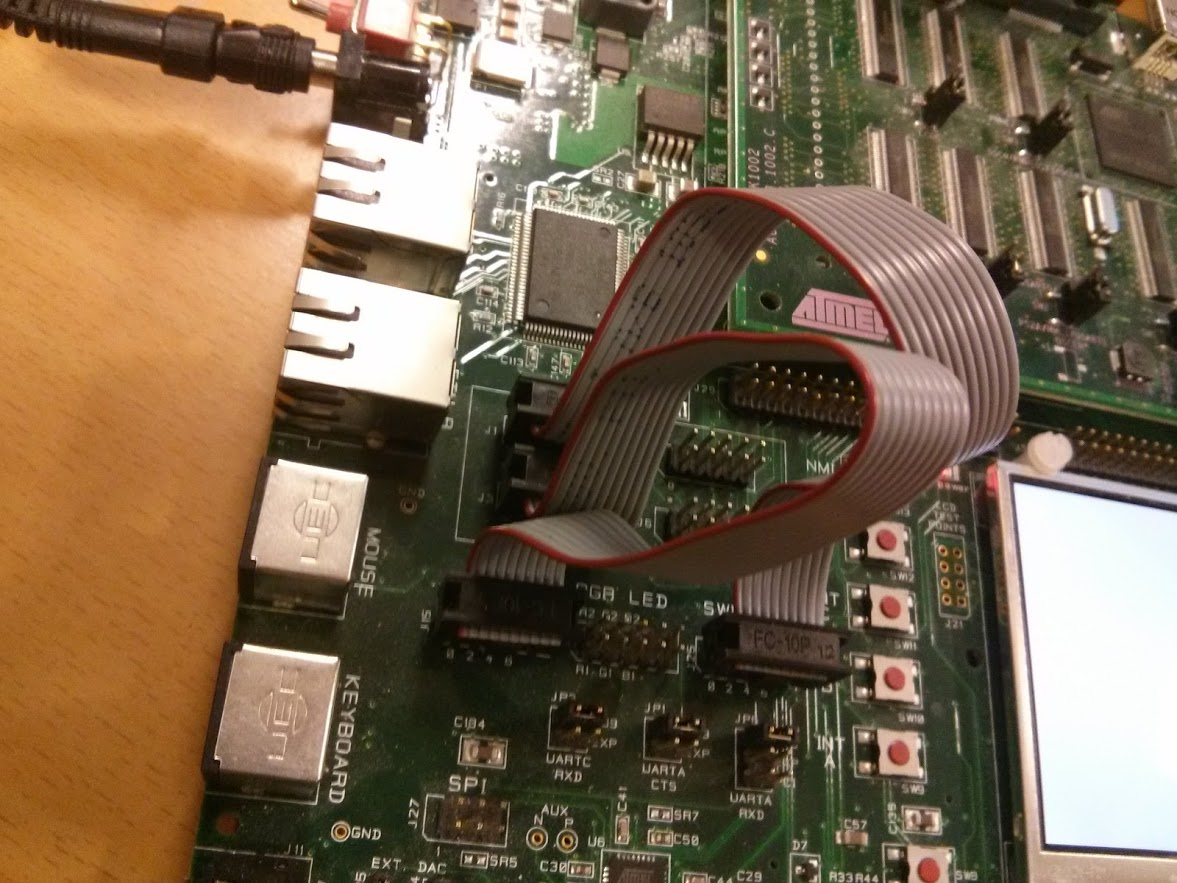
\includegraphics[width = \textwidth]{description-and-methodology/flat-cable-image.jpg}
\caption{Flat cables connecting GPIO with switches and LEDs. Note the orientation of the flat cables.}
\label{flat-cable-image}
\end{figure}


\section{Programming environment}

    \subsection{JTAGICE}

        The AP7000 sisterboard on the STK1000 provides a JTAG interface, which is used for programming and debugging of the board.
The development PC was connected to the JTAG interface of the STK1000 using an Atmel JTAGICE mk II (firmware 7.29).
The JTAGICE does not require external power as long as it is connected to the PC over USB.


    \subsection{GNU Debugger}

        We followed the instructions presented in the compendium in an attempt to employ the GNU debugger, but were confused by the interface as we had not read the recommended further reading material supplied in the compendium.
So we chose to not employ the GNU debugger in the development of our solution.
TODO: run up to the lab and use gdb a bit, so we can write about it here afterwards.


    \subsection{Make}

        GNU Make, a scriptable build tool, was employed in the development of the paddle program.
The handout files included a samle Makefile, which was used mostly without modification.
After the development of the program was complete, and how to use the debugger became clear (see the previous section), a make command to quickly enter debug mode was included.
This command could be invoked by writing \texttt{make debug}.
Aditionally, and somewhat self-referentially, a Makefile for easy compiling of this LaTeX report was used.


    \subsection{Other tools}

        vim, git.


\section{Development of the program}

This section details the steps taken during the development of the program.
Features were added iteratively, starting with simple LED and button integration, and moving on to more sophisticated interrupt-oriented logic/program flow.
The first piece of code written simply enabled all the LEDs and turned them on. Once the LEDs were working, buttons were enabled.
The next step was to write code to turn on just one of the LEDs, designated the ''paddle'' per the assignment's description (\cite{lab-compendium}, pg 37).

Code was written to move the paddle right when \texttt{SW0} was pushed, and left when \texttt{SW2} was pushed, employing arithmetic shift to move the paddle bit in the appropriate direction.
However, a single push of either button caused the paddle to disappear.
This was due to a combination of the paddle's bit overflowing when it reached either edge, making the paddle disappear, and the fact that a single button press was registered many, many times.
The latter happened because a button press was registered for each iteration of the program's main loop while a button was held down.
The code was altered so that the paddle would loop around to the opposite side of the row of LEDs when it was pushed off either side.

At this point, when pushing either buttons, all the LEDs would light up briefly in turn at such high a speed that it looked like they were all dimly lit simultaneously.
This is again because of the massive amount of times the main loop would iterate whilst a button was pressed, causing the paddle to cycle the LED row at break-neck speeds.
Implementing some sort of button cool-down to reduce the frequency of registered button presses would be the next step if we wanted to continue working with the polling approach to button handling, but we opted rather to migrate to an interrupt-based approach.
This choice had the benefit of making the program more energy efficient, as well as it being a hard requirement of the assignment.
Implementing interrupts for the buttons introduced hardware bouncing problems, which were solved by implementing software debouncing (\cite{lab-compendium}, Fig. 2.9a).

An issue arised where the paddle would move over one additional LED when a button was pushed (i.e. from \texttt{LEDn} to \texttt{LEDn+2} rather than from \texttt{LEDn} to \texttt{LEDn+1}).
This was caused by the fact that lifting a button from a pressed state to an unpressed state generated an unwanted interrupt.
This was fixed by ignoring every second registered push of each button.

    \subsection{Setting up the LEDs}
        
        The connection to the output LEDs must be set up before the LEDs can be used in a program.
First, the I/O pins that the LEDs are connected to must be enabled.
In this assignment, the LEDs are connected to the pins GPIO16-23, corresponding to PIO C lines 0-7.
To enable the correct I/O pins, we must therefore set to 'high' bits 0-7 of the PIO C PIO Enable Register (PIOC PER), as in listing x.
Here, r3 is the base offset of PIOC, AVR32\_PIO\_PER is the PIO Enable Register offset, and r6 contains the bitfield indicating which pins to enable.

\code{99}{100}{Enable the I/O pins}

Second, the I/O pins must be set to act as output pins, as opposed to input pins.
This is done by setting to 'high' the corresponding bits (0-7) of the PIO C Output Enable Register (PIOC OER), as in listing x.
Here, r3 is the base offset of PIOC, AVR32\_PIO\_OER is the Output Enable Register offset, and r6 contains the bitfield indicating which pins to set as outputs.

\code{102}{103}{Set the pins to act as output pins}

Once this is done, LEDs can be turned on by writing the appropriate bits to PIO C Set Output Data Register (PIOC SODR), as in listing x.
Here, r3 is the offset of PIOC, AVR32\_PIO\_SODR is the Set Output Data Register offset, and r4 contains the bitfield indicating which LEDs to switch on.

\code{176}{177}{Switch on LEDs}

Analogously, LEDs can be turned of by writing the approtiate bits to PIO C Clear Output Data Register (PIOC CODR), as in listing x. 
Here, r3 is the offset of PIOC, AVR32\_PIO\_SODR is the Set Output Data Register offset, and r4 contains the bitfield indicating which LEDs to switch off.

\code{173}{174}{Switch on LEDs}


    \subsection{Setting up the buttons}

        The connection to the input buttons must be set up before the buttons can be used in a program.
First, the I/O pins that the buttons are connected to must be enabled.
In this assignment, the buttons are connected to the pins GPIO0-7, corresponding to PIO B lines 0-7.
To enable the correct I/O pins, we must therefore set to 'high' bits 0-7 of the PIO B PIO Enable Register (PIOB PER), as in <code excerpt>.

    st.w r2[AVR32_PIO_PER], r6


    <code excerpt>: Here, r2 is the base offset of PIOB, AVR32_PIO_PERhis the PIO Enable Register offset, and r6 contains the bitfield indicating which pins to enable.


Second, the pull-up resistors for the buttons must be enabled. This is because <reason>.
This is done by setting to 'high' the corresponding bits (0-7) of the PIO B Pull-Up Enable Register (PIOC PUER), as in <code excerpt>.

    st.w r2[AVR32_PIO_PUER], r6

    <code excerpt>: Here, r2 is the base offset of PIOB, AVR32_PIO_PUER is the Pull-Up Enable Register offset, and r6 contains the bitfield indicating which pull-up resistors should be enabled.


Once this is done, the button state can be read by reading the appropriate bits from PIO B Pin-Data Status Register (PIOB PDSR), as in <code excerpt>.

    ld.w r12, r2[AVR32_PIO_PDSR]
    
    <code excerpt>: Here, r2 is the offset of PIOB, AVR32_PIO_PDSR is the Pin-Data Status Register offset.



    \subsection{Setting up the interrupts}

        Before interrupts can be utilized we have to configure the board in an appropriate manner. This process is outlined in section 2.5 of \cite{lab-compendium}.
\subsubsection{Enabling Interrupts}
Since we connected the buttons to PIO port B, we will be detailing how we enabled interrupts from PIO port B.
First, we set the appropriate bits in the Interrupt Enable Register to 1, see listing 8, 9 and 10.
\code{84}{84}{The base address of PIO port B is loaded into r2.}
\code{97}{97}{The masks of Button 0 and Button 2 are loaded into r5}
\code{114}{115}{Interrupts are enabled for Button 0 and Button 2}
Before we enable interrupts for Button 0 and Button 2, we defensively disable interrupts for everything by loading \texttt{0xff} into the Interrupt Disable Register.
Finally, then enable interrupts globally by setting the bit GM (Global Interrupt Mask) in the processor's status register to 0 (see listing 11) % taken from pg 26 of the compendium
\code{126}{127}{Enable interrupts globally.}
% EVBA = Exception Vector Base Address
\subsubsection{Loading the interrupt routine}
After enabling interrupts, we have to inform the processor about what to do when it receives an interrupt.
First, we specify the address of our interrupt routine to be used as the autovector when the interrupt controller receives an interrupt from group 14. The code for this is displayed in listing 12, 13 and 14.
\code{86}{86}{The base address of the interrupt controller is loaded into r7.}
\code{87}{87}{The address of our interrupt routine is loaded into r8.}
\code{120}{121}{The address of our interrupt routine is stored in IPR14's register in the interrupt controller.}
Then we have to set the processor's EVBA\footnote{Exception Vector Base Address} register to the desired value, i.e. zero (see listing 15).
\code{117}{118}{Setting the EVBA to 0. 0 is stored in r1.}
This is because the interrupt routine address is calculated by adding together the EVBA and autovector, where the autovector is represented by the 14 least significant bits in the interrupt routine address.
By setting the EVBA to 0, the interrupt routine address simply becomes the autovector, which we have specified as the address of our interrupt routine.


    \subsection{Interrupt Routine}

        Our interrupt routine first reads the state of the buttons by calling another routine which stores the buttons' state in \texttt{r12}.
\code{190}{191}{Read button state.}
Once the buttons' state has been read, the debouncing routine (\cite{lab-compendium}, Figure 2.9a) is called to prevent bouncing. 
\code{193}{194}{Debounce!}
Wthat \texttt{0xfff} 


%% EXECUTIVE SUMMARY
The button interrupt routine first reads the state of the buttons before calling a debounce routine which runs for some amount of time.
When the debounce routine is finished the button interrupt routine notifies that the interrupt has been handled before returning to the main loop.
\\ % starts a new paragraph
The debounce routine's running time can be modified by altering the DEBOUNCE constant, which can be considered the routine's loop counter. The routine keeps the CPU busy by repeatedly subtracting one from this value until it reaches zero. This prevents further interrupts from being registered for the duration of the debouncing routine.

%% full blown deets.
In order to implement an interrupt routine we have to enable the relevant interrupts and tell the interrupt controller where it can find the interrupt routine.
Interrupts are enabled for specific I/O units by loading the appropriate values into the Interrupt Enable Register.
We want to enable interrupts for SW0 and SW2.
Their masks are \texttt{0x1} and \texttt{0x4}, respectively.


We enable interrupts by loading the appropriate values into the Interrupt Enable Register (PER).
Specifically, the \"appropriate values\" are the masks for SW0 and SW2, which are \texttt{0x1} and \texttt{0x4}, respectively.
Since our buttons are connected to PIOB, we load the masks
More specifically, we load these masks into a register, and then 
\\*
We load PIO B's base address into r2
\texttt{
		/* */
		lddpc r2, piob_offset
		/* The masks of SW_0 and SW_2 are loaded into r5 */
		mov r5, SW_0 | SW_2
		/* */
		st.w r2[AVR32_PIO_IER], r5
}
% store the mask of SW0 and SW2 in r5

% starts a new line, but not a new paragraph
% PIO_IER is the interrupt enable register
\texttt{st.w r2[AVR32_PIO_IER], r5 }

This is done by storing the appropriate values in the PIO Enable Register (PER).
We enabled button interrupts for \texttt{SW0} and \texttt{SW2} by loading their masks into the PIOB, with the appropriate offset to specify
GPIO pins = PIO
general purpose input/output pins

% load the pointer to PIOB's base address into r2
lddpc r2, piob_offset
% load the pointer to the interrupt controller's base address into r7
lddpc r7, intc_base
% store the address of the interrupt routine in r8
mov r8, button_interrupt_routine
% store the mask of SW0 and SW2 in r5
mov r5, SW_0 | SW_2
% enable button interrupts for SW0 and SW2
% PIO_IER is the interrupt enable register
st.w r2[AVR32_PIO_IER], r5 
% stores the address of our button interrupt routine in the interrupt controller
st.w r7[AVR32_INTC_IPR14], r8

\texttt{st.w r2[AVR32_PIO_IER], r5}
Enables button interrupts for SW0 and SW2.
First, interrupts must be disabled


lddpc r7, intc_base
% intc_base is a pointer to the address of the interrupt controller

mov r8, button_interrupt_routine
% the address of the interrupt routine is loaded into r8

st.w r7[AVR32_INTC_IPR14], r8
% the address of the interrupt routine is stored in the interrupt controller's button h

The time is specified 
First the state of the buttons is read.
The debounce routine simply waits for a time decided by the DEBOUNCE constant in CONFIGURATION.

st.w rd, rs
% writes the value in rs to the address found in rd


et spesielt minneområde som skal inneholde adressen til en rutine som vil bli kjørt når kortet mottar en relevant interrupt. I dette tilfelle er relevante interrupts knappe-interrupts.

rcall read_buttons
rcall debounce

ld.w r0, r2[AVR32_PIO_ISR]

rd, rs

rete


    \newpage

    \subsection{Program flow}

        <diagrams, descriptions>

yuml.me-source for diagrams

Main program flow:
(start)->(Init)->(Main loop)->(Main loop)


Init:
(start)->(Load pointers)->(Set up start values in registers)->(Enable I/O with interrupts)->(end)

Main loop:
(start)->(Set leds)->(Sleep)[interrupt]-><interrupt routine>->[Was SW0 pressed][Yes]->(Move paddle right)->(end),[Was SW0 pressed][No]->(Move paddle left)->(end)


Set leds:
(start)->(Turn off all LEDs)->(Turn on the paddle LED)->(end)

Button interrupt routine:
(start)->(Read button states)->(Software debounce)->(Notify that the interrupt has been handled)->(end)

Debounce:
(start)->(Set register to a high constant)->(Is value in register equal to 0)[Yes]->(end),(Is value in register equal to 0)[No]->(Decrease value in register by 1)->(Is value in register equal to 0)

Read buttons:
(start)->(Read button status)->(Mask away buttons that were pressed in previous interrupt)->(end)

Move paddle right:
(start)->(Is paddle at far-right end of the board)[Yes]->(Move paddle to far-left)->(end),(Is paddle at far-right end of the board)[No]->(Move paddle one step to the left)->(end)

Move paddle left (analogous to move paddle right, but included for completeness):
(start)->(Is paddle at far-left end of the board)[Yes]->(Move paddle to far-right)->(end),(Is paddle at far-left end of the board)[No]->(Move paddle one step to the right)->(end)



        \newpage

    \subsection{Register Overview}

        The STK1000 has 13 general purpose registers named r0-r12. The programmer is free to use these registers for whatever they want.
However, several conventions are commonplace to introduce a certain degree of structure.

Conventions:

r0 is a scratch register, used for intermediate calculations and such.
r1 holds the constant 0.

...

r8, r9, r10, r11, r12:

used to hold parameters when calling a routine.

r12:

used to hold the return value when returning from a routine.


List of registers and what they are used for in the paddle move program:

\begin{center}
\begin{table}
    \begin{tabular}{|l|l|}
        r0  & Scratch register used to hold intermediate values. \\
        r1  & Constant: 0 \\ 
        r2  & Constant: base offset to PIOB \\ 
        r3  & Constant: base offset to PIOC \\ 
        r4  & Variable: holds the position of the paddle \\ 
        r5  & Constant: 5 \\ 
        r6  & Constant: 0xff \\ 
        r7  & Variable: holds the previous button state \\ 
        r8  & Constant: pointer to button interrupt routine \\ 
        r9  & (not used) \\ 
        r10 & (not used) \\ 
        r11 & (not used) \\ 
        r12 & Holds return value from routines \\
    \end{tabular}
\label{tab:label}
\end{table}
\end{center}


